\documentclass[UTF8]{ctexart}
\CTEXsetup[format={\Large\bfseries}]{section}
\usepackage{amssymb}
\usepackage{amsmath}
\usepackage{cases}
\usepackage{ulem}
\usepackage{geometry}
\usepackage{multirow}
\usepackage{graphicx}
\usepackage{diagbox}
\usepackage{amssymb}
\usepackage{amsmath}
\usepackage{cases}
\usepackage{ulem}
\usepackage[colorlinks,linkcolor=blue]{hyperref}
\usepackage{enumerate}
\usepackage{listings,xcolor}
\usepackage{color}
\definecolor{dkgreen}{rgb}{0,0.6,0}
\definecolor{gray}{rgb}{0.5,0.5,0.5}
\definecolor{mauve}{rgb}{0.58,0,0.82}
\usepackage{subfigure}

\lstset{
frame=tb,
language=Java,
tabsize = 4, %% set tab space width
showstringspaces = false, %% prevent space marking in strings, string is defined as the text that is generally printed directly to the console
numbers = left, %% display line numbers on the left
commentstyle = \color{green}, %% set comment color
keywordstyle = \color{blue}, %% set keyword color
stringstyle = \color{red}, %% set string color
rulecolor = \color{black}, %% set frame color to avoid being affected by text color
basicstyle = \small \ttfamily , %% set listing font and size
breaklines = true, %% enable line breaking
numberstyle = \tiny,
}

\lstset{frame=tb,
  language=Python,
  aboveskip=3mm,
  belowskip=3mm,
  showstringspaces=false,
  columns=flexible,
  basicstyle={\small\ttfamily},
  numbers=none,
  numberstyle=\tiny\color{gray},
  keywordstyle=\color{blue},
  commentstyle=\color{dkgreen},
  stringstyle=\color{mauve},
  breaklines=true,
  breakatwhitespace=true,
  tabsize=3
}
%算法包
\usepackage{caption}
\usepackage{algorithm,float}
\usepackage{algorithmic}
\usepackage{blindtext}
% Page header
\usepackage{fancyhdr} % Headers and footers
\pagestyle{fancy} % All pages have headers and footers
\fancyhead{}\renewcommand{\headrulewidth}{0pt} 
%算法input output
\renewcommand{\algorithmicrequire}{\textbf{Input:}} % Use Input in the format of Algorithm
\renewcommand{\algorithmicensure}{\textbf{Output:}} % Use Output in the format of Algorithm
\DeclareMathOperator*{\argminA}{arg\,min} % Jan Hlavacek

\usepackage{tabu}

\geometry{a4paper,scale=0.85}
\begin{document}
\fancyhead[C]{}
\hrule \medskip % Upper rule
\begin{minipage}{0.295\textwidth} 
\raggedright
\footnotesize
崔子寒 \hfill\\   
MG20330012 \hfill\\
zihancui@smail.nju.edu.cn
\end{minipage}
\begin{minipage}{0.4\textwidth} 
\centering 
\large 
Assignment 2: jmtrace\\ 
\normalsize 
ISER,20\\ 
\end{minipage}
\begin{minipage}{0.295\textwidth} 
\raggedleft
\today\hfill\\
\end{minipage}
\medskip\hrule 
\bigskip

\section{Java字节码插桩}
为了获得更好的跨平台特性,Java的源代码会被编译成特定的字节码,再由JVM来解释执行。JVM的输入就是Java源代码编译产生的字节码,每一个类都会被编译成一个.class文件,当我们执行Java代码时,JVM会将所需的.class文件中类的信息加载入内存,并解析生成对应的class对象。这个过程被称为Java的类加载,实际上JVM要做的事情非常复杂,但是我们只需要知道我们可以捕捉这个加载过程,并修改即将加载入内存中的类的字节码,在我们关心的指令前后插入一些新的指令,这就是Java字节码插桩的原理。
\section{插桩实现}
\subsection{Java Instrument和Java ASM}
为了方便开发者捕捉类的加载过程,java提供了\texttt{java.lang.instrument}包,其中的\texttt{Instrumentation}类提供了在类加载过程中修改类的字节码的方法。当我们运行一个jar包时,如果设定了它的javaagent,那么JVM就会在加载jar之前先加载javaagent,并执行它的\texttt{preMain}方法。在\texttt{preMain}方法中,我们会调用\texttt{Instrumentation}类的\texttt{addTransformer}方法,传入一个实现了\texttt{ClassFileTransformer}接口的对象。然后会通过运行该对象的\texttt{transform}方法来完成插桩,所以我们的任务主要是编写一个实现了\texttt{ClassFileTransformer}接口的类。

直接在\texttt{transform}方法中解析字节码工作量比较大,我们可以利用一些开源的包,比如Java ASM。Java ASM提供了两套不同风格的API用于插桩,分别是基于事件的Core API和基于对象的Tree API。两套API的功能是等价的,我们采用Core API来实现插桩。
\subsection{理解相关JVM指令}
在插桩之前,首先需要理解JVM中的一些特性,最重要的一点是JVM的指令集是基于栈而不是基于寄存器的。对于需要参数的指令,都是在执行指令之前将参数放入栈中,指令执行时从栈中取出参数,指令执行结束后,将结果再压入栈中,函数的调用也是类似。

JVM中的数据类型再栈中有两种。category 1在栈中的长度是1个单位,category 2在栈中的长度是2个单位,只有\texttt{double}和\texttt{long}是category 2。在插桩的实现中,我们需要针对不同的数据类型,使用不同的指令。


\subsection{实现插桩}
在\texttt{transform}方法中,我们读取类的字节码,然后用一个visitor按照指令的顺序遍历字节码,当读到目标的指令时,就进行插桩,最后将插桩完的字节码返回。
\begin{lstlisting}[language=Java]
    ClassReader reader = new ClassReader(classfileBuffer);
    ClassWriter writer = new ClassWriter(reader, ClassWriter.COMPUTE_MAXS);
    ClassVisitor visitor = new MemoryTraceClassVisitor(writer);
    reader.accept(visitor, 0);
    return writer.toByteArray();
\end{lstlisting}
在visitor中,我们根据读到的指令类型以及opcode来检查是否读到了我们的目标指令,如果读到,就调用相关的方法进行插桩。我们的目标指令是\texttt{*aload/*astore/getfield/putfield/getstatic/putstatic},我们需要获取这些指令执行时有关的对象的信息,有关线程的信息等,一个比较好的方法是获取对象的引用,以及相关的变量,并将它们作为参数放入栈中,然后插入调用我们自己写的打印信息的方法的指令。\ref{fig:lastore}展示了如何对\texttt{lastore}指令实现上面的过程。
\begin{figure}[htbp]
    \centering
    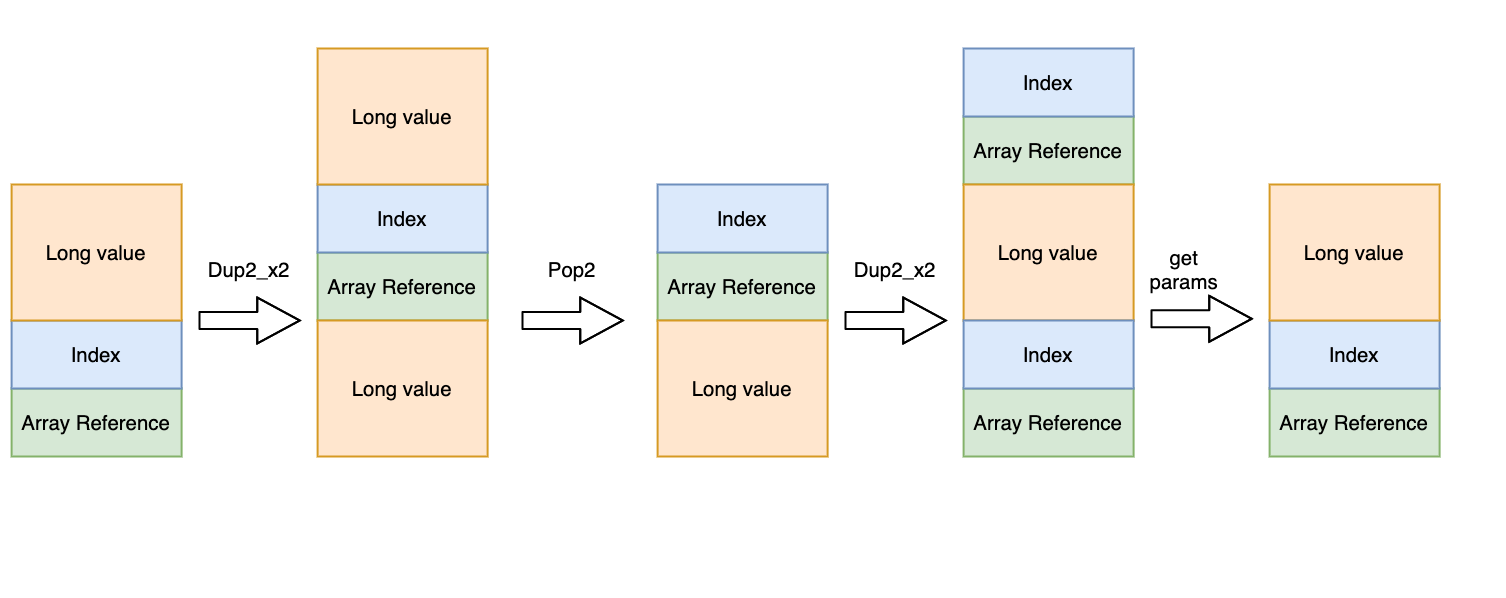
\includegraphics[width=5in]{lastore.png}
    \caption{lastore instrument}
    \label{fig:lastore}
\end{figure}

需要注意的一点是,对于\texttt{putfield}指令,我们直接通过指令是无法判断栈中的value是category 1还是category 2,所以需要通过反射获取相关的对象的类型,然后再分情况进行操作:
\begin{lstlisting}[language=Java]
    final Type fieldType = Type.getType(descriptor);
    if(fieldType.getSize() == 1) {
        // value is category 1
        mv.visitInsn(Opcodes.DUP2);
        // [...,objRef, value, objRef, value] <-
        mv.visitInsn(Opcodes.POP);
        // [...,objRef, value, objRef] <-
    } else {
        // value is category 2
        mv.visitInsn(Opcodes.DUP2_X1);
        // [...,value, objRef, value] <-
        mv.visitInsn(Opcodes.POP2);
        // [...,value, objRef] <-
        mv.visitInsn(Opcodes.DUP_X2);
        // [...,objRef, value, objRef] <-
    }
\end{lstlisting}
在准备好了参数之后,只需要调用我们的方法,就可以完成插桩:
\begin{lstlisting}
    // [..., objRef, value, objRef] <-
    mv.visitLdcInsn(owner);
    // [..., objRef, value, objRef, ownerStringRef] <-
    mv.visitLdcInsn(name);
    // [..., objRef, value, objRef, ownerStringRef, nameStringRef] <-
    mv.visitMethodInsn(Opcodes.INVOKESTATIC, Type.getInternalName(MemoryTraceUtils.class), "tracePutField", "(Ljava/lang/Object;Ljava/lang/String;Ljava/lang/String;)V", false);
    // [..., objRef, value] <-
\end{lstlisting}
\end{document}

